
\chapter{Turbulence} \label{ch:Turbulence}
\graphicspath{{chapter2_ys/}}
\minitoc


Turbulence gives rise to fluctuations of density $\tilde{n}$, temperature $\tilde{T}$, electric potential $\tilde{\phi}$ and magnetic field $\tilde{\bu{B}}$ in fusion plasmas, and therefore has an influence on the confinement performance and the radial transport of energy and particles. In this chapter, first the general properties of turbulence are introduced in section \ref{sec:general_turbulence}. Then, we focus on plasma turbulence in magnetic confinement devices and its effects on the confinement and transport, as discussed in Section \ref{sec:turbulent_transport}. Plasma turbulence in tokamaks is driven by drift wave instabilities, among which TEM and ITG modes play the most important role in the core region, as detailed in Section \ref{sec:drift_wave_turbulence}. Finally, we focus on the properties of density fluctuations $\tilde{n}$ in Section \ref{sec:properties_of_density_fluctuations}.


\section{General properties of turbulence} \label{sec:general_turbulence}

Turbulence is a state of irregular fluid motion (liquids, gases, plasmas). It is a commonly observed phenomenon in both nature and our daily lives, such as water flow around an obstacle, air flow in the atmosphere or around the wing of an aeroplane, smoke from a chimney, etc. Although turbulence is ubiquitous, experimental characterization and computer modeling of the phenomenon are highly complicated due to the nonlinearity, hence strong dependence on initial conditions, and dynamics at multiple length and time scales. A comprehensive theoretical model is still lacking, although various aspects of turbulence have been studied in detail, e.g., the transition from laminar to turbulent flow in liquids \cite{Chu_1993_JFM} or the effects of plasma turbulence on global energy confinement and transport \cite{TFR_1986_NF, Garbet_1992_NF}.


\subsection{Generation of turbulent phenomena} \label{sec:phenomena_of_turbulence}

Considering first a neutral fluid, the onset of turbulence can be characterized empirically by a dimensionless parameter called the \emph{Reynolds number}:%
%%%%%%%%%%%%%%%%%%%%
\begin{equation}\label{eq:Reynolds_number}
  R_e=\frac{uL}{\nu}.
\end{equation}
%%%%%%%%%%%%%%%%%%%%
\noindent Here, $u$, $L$ and $\nu$ denote the fluid velocity, the characteristic linear dimension of the system and the kinematic viscosity, respectively. The Reynolds number can be regarded as the ratio between the inertial forces and the viscous forces in a fluid. At low Reynolds number, when the viscous forces are dominant, the fluid exhibits relatively regular motion, referred to as \emph{laminar flow}. At high Reynolds number, when the fluid motion is typically dominated by inertial forces, a turbulent flow develops because of instabilities driven by the inertial forces. Figure \ref{fig:Reynolds_number} shows an example where a cylinder is positioned in a flowing fluid with varying Reynolds number ($R_e$). When $R_e \gg 1$, turbulent flow appears in the downstream region of the cylinder.


%%%%%%%%%%%%%%%%%%%%
\begin{figure}[h]
\begin{centering}
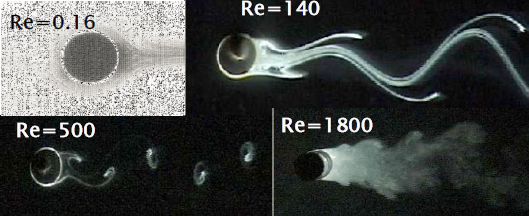
\includegraphics[scale=0.65]{Reynolds_number.png}
\par\end{centering}
\caption[Turbulent flow around a cylinder in a fluid]{Formation of turbulence behind a cylinder placed in a fluid flow, gradually increasing the Reynolds number ($R_e$). The experimental conditions to change the characteristic parameters of $u$, $L$, $\nu$ can be found in \cite{Acheson_1990_Turbulence, Pope_2000_Turbulence}.}
\label{fig:Reynolds_number}
\end{figure}
%%%%%%%%%%%%%%%%%%%%


Historically, Reynolds's dye experiments in 1883 led him to define the Reynolds number as a good indicator of fluid turbulence. However, no clear origins or driving mechanisms of turbulence were proposed following this experimental investigation. Deeper theoretical studies revealed that turbulence is caused by fluid instabilities\footnote{To the turbulent flow in fluids, the main instabilities are the Kelvin-Helmholtz instability and the Rayleigh-Taylor instability.}. From figure \ref{fig:Reynolds_number}, one observes a highly distorted surface that separates regions of turbulent and non-turbulent flow. Regions of turbulent flow are characterized by large vorticity, which describes the local spinning motion of a continuum near some point or in other words the tendency of rotation \cite{Acheson_1990_Turbulence}. In contrast, non-turbulent flow is essentially irrotational. Another feature of turbulence is its intermittency, meaning that at fixed position in a fluid, the motion may at times be irregular and other times non-turbulent \cite{Acheson_1990_Turbulence}. Together, the high irregularity at multiple scales and the intermittent nature call for a statistical description of turbulence.


\subsection{Energy cascade, eddies and vortices} \label{sec:turbulence_generation_and_consequences}

Now consider a fully turbulent flow at high Reynolds number. An important property in turbulence is the appearance of \emph{vortices} \cite{Ting_1991_Vortex}. A vortex is a region in a fluid in which the flow revolves around an axis line with non-vanishing vorticity (curl of the velocity). Once formed, vortices can move, stretch, twist and interact with each other in complicated ways. A moving vortex carries with it momentum, energy, and mass.

In addition, a region of swirling, moderately coherent motion of fluid in a turbulent flow is called an \emph{eddy}. A region occupied by a large eddy can also contain smaller eddies \cite{Pope_2000_Turbulence}, as can be seen in figure \ref{fig:Reynolds_number}. The largest eddies are characterized by a length scale which is comparable to the turbulent flow scale. According to the important concept of Richardson's \emph{energy cascade} \cite{Richardson_1922_Turbulence}, the large eddies are unstable and transfer their energy to smaller eddies. At the smallest scales the Reynolds number is sufficiently small such that viscosity becomes effective in dissipating the kinetic energy \cite{Pope_2000_Turbulence}.

Figure \ref{fig:energy_cascade} illustrates the energy cascade process by means of the wavenumber ($k$) and energy $E(k)$. Large eddies have low wavenumber and small eddies have large wavenumber. The intermediate range of scales is called inertial subrange and has been studied by A. Kolmogorov using self-similarity \cite{Kolmogorov_1941_MPS}. Kolmogorov's hypotheses led to the following universal form for the energy spectrum:%
%%%%%%%%%%%%%%%%%%%%
\begin{equation}\label{eq:energy_cascade}
  E(k) \propto k^{-5/3}, k > k_{inj}.
\end{equation}
%%%%%%%%%%%%%%%%%%%%
\noindent Thus, in a turbulent system energy is injected at large spatial scales (low $k$) and dissipated at small spatial scales (high $k$). This energy transfer from large towards small structures is observed in three-dimensional isotropic turbulence and is usually called the direct cascade. However, in the framework of a two-dimensional anisotropic turbulent system \cite{Kraichnan_1971_JFM}, except for the direct cascade, the energy can also be transferred from small to large scales, called the inverse cascade. In this case, the energy spectrum can be described as:%
%%%%%%%%%%%%%%%%%%%%
\begin{eqnarray}
% \nonumber to remove numbering (before each equation)
  E(k) &=& k^{-5/3}, k < k_{inj}, \\
  E(k) &=& k^{-3}, k > k_{inj}.
\end{eqnarray}
%%%%%%%%%%%%%%%%%%%%
\noindent Here, a knee point ($k=k_{inj}$) appears in the energy spectrum. Note that in plasma turbulence observed experimentally, the situation can be even more complicated and several injection scales can coexist simultaneously, leading to possible changes of the spectral indices. The energy spectrum will be useful to determine the main contributions to the turbulence signals in the remainder.

Due to the formation of eddies and vortices in turbulent flow, energy and particles exhibit additional transverse motions which enhances the rate of energy and momentum exchange between different regions of the flow. This increases heat transfer, particle transport and friction coefficient. In fact, in engineering applications, most systems with fluid motion are in a turbulent regime rather than a stable state. In these systems, energy and particle transport is dominated by turbulent transport rather than collisional transport. Turbulence and the resulting enhanced transport can be harmful or beneficial, depending on the situation.


%%%%%%%%%%%%%%%%%%%%
\begin{figure}[h]
\begin{centering}
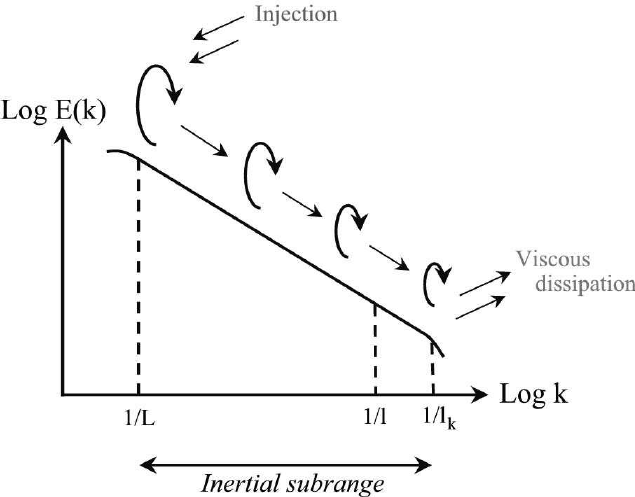
\includegraphics[scale=0.4]{energy_cascade.png}
\par\end{centering}
\caption[Schematic illustration of the energy cascade process of turbulence]{Schematic illustration of the energy cascade process of turbulence. The energy injection and viscous dissipation occur at large (low $k$) and small (high $k$) scale, respectively. Here, the energy injection occurs at $k_{inj} \sim 1/L$. Adapted from \cite{Frish_Cambridge_Turbulence}.}
\label{fig:energy_cascade}
\end{figure}
%%%%%%%%%%%%%%%%%%%%


\section{Turbulent transport in magnetically confined fusion plasmas} \label{sec:turbulent_transport}

In analogy with fluids, in MHD theory fusion plasmas are considered as quasi-neutral fluids of charged particles subject to hydrodynamic and electromagnetic forces. Under certain conditions, fusion plasmas exhibit turbulence, involving irregular, self-regulating structures and dynamics, causing energy \cite{Wootton_1990_PoF, Rice_2012_PoP} and particle transport \cite{Angioni_PPCF_09_review_particle_transport} to be dominated by turbulent transport rather than collisional transport. Here, the same two-edged situation may occur for fusion plasma turbulence. Although plasma turbulence can be advantageous to lessen impurity accumulation in the core region in fusion devices, it is deleterious to the confinement performance by increasing the loss rate of energy and particles. Therefore, understanding and controlling plasma turbulence is a key research topic in fusion science. In this section, we focus on magnetically confined fusion plasmas and the turbulence-related energy and particle transport, as well as different confinement regimes..


\subsection{Turbulence-induced confinement degradation} \label{sec:turbulence_degrades_confinement}

The most straightforward way to demonstrate the link between turbulence and transport in fusion plasmas is to build a relation between the characteristics of the turbulence level and the energy confinement time. The global energy confinement time is defined as the typical time it would take for the plasma energy to leave the system through transport processes (not accounting for radiation), if all heating sources were suddenly switched off. It is calculated as the ratio of the total stored plasma energy over the power lost through the separatrix.

%%%%%%%%%%%%%%%%%%%%
\begin{figure}[h]
\begin{centering}
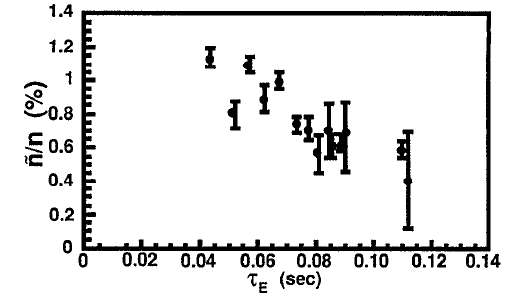
\includegraphics[scale=0.65]{tau_vs_dn.png}
\par\end{centering}
\caption{Turbulence level ($\widetilde{n}/n$) measured from beam emission spectroscopy (BES) versus the energy confinement time ($\tau_E$) for an Ohmic discharge in TFTR. Adapted from \cite{Paul_1992_PoF}.}
\label{fig:tau_vs_dn}
\end{figure}
%%%%%%%%%%%%%%%%%%%%

Quantitative analyses of the turbulence level and the confinement time have been carried out through power scans in many tokamaks such as TFR (Tokamak de Fontenay-aux-Roses) \cite{TFR_1986_NF} and TFTR (Tokamak Fusion Test Reactor) \cite{Paul_1992_PoF}. In TFR, The analyses have been conducted with ICRH and NBI and a negative correlation between the turbulence level and the confinement time was observed. In TFTR, the similar trend, i.e., the global energy confinement time ($\tau_E$) is approximately inversely proportional to the density fluctuation level ($\widetilde{n}/n$), was recovered in Ohmically heated plasmas, as shown in figure \ref{fig:tau_vs_dn}. These results (together with many confirms from other devices) indicate that turbulence indeed plays a major role in determining the confinement time.


\subsection{Heat transport} \label{sec:heat_transport}

One way to quantify the relation between turbulence and transport is to experimentally determine the corresponding effective heat transport coefficients. The effective heat transport coefficient $\chi_s$ is defined through the following formula:%
%%%%%%%%%%%%%%%%%%%%
\begin{equation}\label{eq:heat_transport}
  \bu{q_s}=-n_s\chi_s{\nabla}T_s,
\end{equation}
%%%%%%%%%%%%%%%%%%%%
\noindent with $\bu{q_s}$, $n_s$ and $T_s$ the heat flux vector, density and temperature of each specific species $s$. The heat transport coefficient of electron and ions ($\chi_e$ and $\chi_i$) can be estimated experimentally, roughly resulting in $\chi_e^{exp} \sim \chi_i^{exp} \sim 1m^2s^{-1}$.

%%%%%%%%%%%%%%%%%%%%
\begin{figure}[h]
\begin{centering}
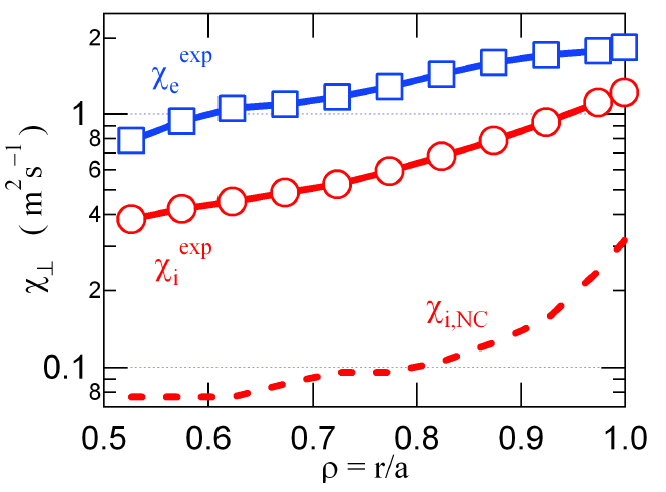
\includegraphics[scale=0.55]{heat_transport_coefficient.png}
\par\end{centering}
\caption{Experimental estimates of electron and ion heat transport coefficients and neoclassical value from the tokamak Tore Supra. From \cite{Sarazin_cours}.}
\label{fig:heat_transport_coefficient}
\end{figure}
%%%%%%%%%%%%%%%%%%%%

On the other hand, Coulomb collisions also contribute to the radial transport. Transport in a toroidal geometry is described by neoclassical transport theory, considering the inhomogeneity of the magnetic fields and the population of trapped particles (figure \ref{fig:trapped_particles}). The precise derivation of the neoclassical transport coefficients in the different collisional regimes can be found in \cite{Hinton_1976_RMP}. They can be related to the corresponding coefficients in classical cylindrical geometry, as follows:%
%%%%%%%%%%%%%%%%%%%%
\begin{equation}
  \chi_s^{NC} \sim q^2(r/R)^{-3/2}\chi_s^{C}, s=e,i.
\end{equation}
%%%%%%%%%%%%%%%%%%%%
\noindent Here, $q$ is the safety factor, $r$ the radial position in a poloidal cross-section and $R$ the major plasma radius. The classical coefficients are given by $\chi_e^C \sim \nu_{ee}\rho_e^2$ and $\chi_i^C \sim \nu_{ii}\rho_i^2$, where $\nu_{ee}$ ($\nu_{ii}$) and $\rho_e$ ($\rho_i$) are the electron (ion)  collision frequency and Larmor radius. The transport spatial scale of neoclassical theory is the width of the banana orbit, which is much larger than the classic Coulomb collision scale (the Larmor radius). This explains why neoclassical transport is stronger than the corresponding classical transport.

The experimentally determined transport coefficients ($\chi_i^{exp}$, $\chi_e^{exp}$) and the theoretical prediction from neoclassical theory ($\chi_i^{NC}$) are shown in figure \ref{fig:heat_transport_coefficient} for a Tore Supra discharge. The experimental estimates are still much larger than those obtained from neoclassical theory, at all the radial positions. Numerous experiments indicate that $\chi_i^{exp} \gg \chi_i^{NC}$ and $\chi_e^{exp} \gg \chi_e^{NC}$. The large unexpected transport coefficients observed experimentally thus can not be explained by any collision-based theory and is conventionally referred as \emph{anomalous transport}, which is believed to be caused by turbulence.


\subsection{Particle transport} \label{sec:particle_transport}

After evaluating the influence of turbulence on energy confinement, now we focus on another important transport in fusion plasmas: particle transport. Particle transport is a central question due to the fact that fusion power increases as the square of the density, so the existence and nature of any process that leads to density peaking deserves attention \cite{Garbet_ITGTEM_2004_PPCF_EPS}. The degree of density peaking is also useful to self-generate a large fraction of non-inductive current required for continuous operation \cite{Bourdelle_PPCF_05_review_turbulent_particle_transport}.

Particle transport in tokamaks is different from heat transport, since the heat source is usually located in the core region but the particle source is often only located in the edge region. Nevertheless, density profiles can still be peaked in the central region due to an inward particle pinch. Therefore, the particle transport flux includes a diffusive and a convective (pinch) term:%
%%%%%%%%%%%%%%%%%%%%
\begin{equation}\label{eq:particle_flux}
  \boldsymbol{\Gamma} = -D\nabla n + \bu{V}n.
\end{equation}
%%%%%%%%%%%%%%%%%%%%
\noindent Here, $n$ is the local density, $D$ the diffusion coefficient and $\bu{V}$ the pinch velocity. In terms of generation mechanism, the particle flux $\boldsymbol{\Gamma}$ can be divided into two parts:%
%%%%%%%%%%%%%%%%%%%%
\begin{equation}\label{eq:neo_flux_and_turb_flux}
  \boldsymbol{\Gamma} = \boldsymbol{\Gamma}_{neo} + \boldsymbol{\Gamma}_{turb},
\end{equation}
%%%%%%%%%%%%%%%%%%%%
\noindent where $\boldsymbol{\Gamma}_{neo}$ and $\boldsymbol{\Gamma}_{turb}$ are generated by the neoclassical transport and the turbulence, respectively. Here, we assume there is no coupling effect between the two terms. The neoclassical part is attributed to the Ware pinch \cite{Ware_1970_PRL}, causing the trapped particles with density $n_t$ to move towards the magnetic axis with a radial velocity $V_{neo}$, satisfying:%
%%%%%%%%%%%%%%%%%%%%
\begin{equation}\label{eq:neo_flux}
  \boldsymbol{\Gamma}_{neo} = \bu{V}_{neo}n_t,
\end{equation}
%%%%%%%%%%%%%%%%%%%%
\noindent with
%%%%%%%%%%%%%%%%%%%%
\begin{equation}\label{eq:Vneo}
  \bu{V}_{neo} = -\frac{E_{\phi}}{B_{\theta}}\bu{e_r},
\end{equation}
%%%%%%%%%%%%%%%%%%%%
\noindent with $\bu{e_r}$ the unit vector in the radial direction. Here, $E_{\phi}$ and $B_{\theta}$ are the magnitude of the toroidal electric field and the poloidal magnetic field, respectively. The anomalous part of the particle flux caused by turbulence can be written as \cite{Bourdelle_PPCF_05_review_turbulent_particle_transport}:%
%%%%%%%%%%%%%%%%%%%%
\begin{equation}\label{eq:turb_flux}
  \boldsymbol{\Gamma}_{turb} = -D_{turb}{\nabla}n + \bu{V}_{turb}n,
\end{equation}
%%%%%%%%%%%%%%%%%%%%
\noindent where $\bu{V}_{turb}$ is the turbulent pinch velocity, $D_{turb}$ is the turbulent diffusion coefficient, and $n$ is the density. There are two main mechanisms that contribute to $\boldsymbol{\Gamma}_{turb}$: the turbulence equipartition (TEP) and the thermodiffusion. TEP is related to the geometric effect of magnetic fields. It is found that the density of trapped particles is inversely proportional to $q$. Since $q$ increases from the core to the edge, a peaked profile forms. The thermodiffusion term predicts a velocity pinch when ($\nabla T/T$)/($\nabla n/n$) is sufficiently high. The existence of the turbulent pinch velocity has been proved experimentally in modulated Tore Supra discharges, as shown in figure \ref{fig:pinch_velocity} \cite{Hoang_2003_PRL_turb_pinch}. The inward pinch velocity $\bu{V}$ from the peaked density profile can only be explained by a turbulent pinch, as the poloidal electric field hence the neoclassical Ware pinch are kept at zero in these shots.

%%%%%%%%%%%%%%%%%%%%
\begin{figure}[h]
\begin{centering}
\includegraphics[scale=0.5]{pinch_velocity.png}
\par\end{centering}
\caption{The pinch velocity ($V$) and the diffusion coefficient ($D$) calculated from the density profile when the neoclassical contribution remains small. This has been realized by long-pulse LHCD discharges with zero toroidal electric field $E_{\phi}$ \cite{Hoang_2003_PRL_turb_pinch}.}
\label{fig:pinch_velocity}
\end{figure}
%%%%%%%%%%%%%%%%%%%%


\subsection{Confinement regimes} \label{sec:confine_regime}

The effects of turbulence on confinement and transport depend on confinement regime. The various confinements regimes can be achieved by adapting global plasma parameters and external heating power. Optimization of confinement performance and exploration of suitable confinement regimes constitutes a central topic in fusion science.


\subsubsection*{\emph{Ohmic confinement regime}}

When only Ohmic heating is applied to the plasmas, it is said to be in the Ohmic confinement regime. In this regime, the relation between the confinement time and the density has been studied extensively \cite{Yushmanov_1999_NF}. At low densities, the confinement time $\tau_{E}$ increases linearly with the increase of the density, characterizing the so-called \emph{linear Ohmic confinement} (LOC). Above a critical density threshold, the confinement time $\tau_{E}$ saturates, reaching the \emph{saturated Ohmic confinement} (SOC) regime. Figure \ref{fig:loc_soc} shows the energy confinement time as a function of average electron density for a series of Ohmic discharges, exhibiting a clear transition from LOC to SOC as density increases. In between the two regimes, a transition regime exists. The saturation of the confinement in the SOC regime may be linked to different regimes of micro-instabilities, as discussed in the next section.

%%%%%%%%%%%%%%%%%%%%
\begin{figure}[h]
\begin{centering}
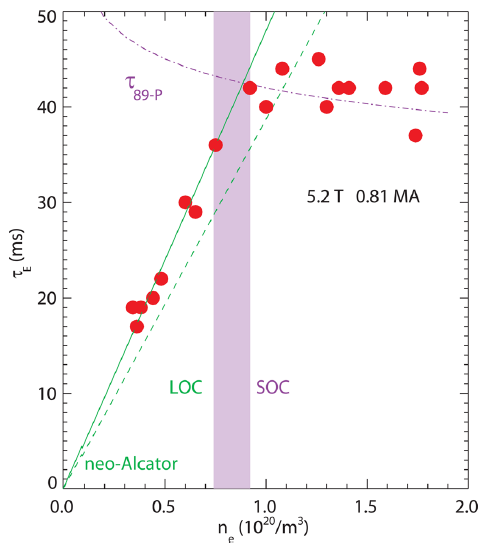
\includegraphics[scale=0.6]{loc_soc.png}
\par\end{centering}
\caption[Energy confinement time as a function of the central line-averaged density]{Energy confinement time as a function of the central line-averaged electron density. Adapted from \cite{Rice_2012_PoP}.}
\label{fig:loc_soc}
\end{figure}
%%%%%%%%%%%%%%%%%%%%


\subsubsection*{\emph{L-mode confinement}}

As the effectiveness of Ohmic heating decreases for increasing temperatures (decreasing plasma resistivity), additional heating methods are required to increase the plasma energy content beyond that obtained with Ohmic heating. This can be achieved by injecting energetic neutral particles or radio-frequency waves. At relatively low levels of auxiliary heating power, it was found that the confinement time decreases with heating power---a regime referred to as the \emph{low confinement mode} (L-mode). Studying L-mode physics is important to increase understanding of turbulent transport and confinement, hence providing useful information for reaching and maintaining H-mode.


\subsubsection*{\emph{H-mode and other improved confinement regimes}}

It was found that tokamak operation makes an abrupt transition from the low confinement mode (L-mode) to the \emph{high confinement mode} (H-mode) when the auxiliary heating power reaches a critical value with the diverter in X point configuration. The underlying physical mechanisms of the L-H transition are still unclear, but it is known to be related to the suppression of turbulent transport \cite{Shaing_1990_PoF, Groebner_1990_PRL, Manz_2012_PoP, Schmitz_2012_PRL}. Empirical scaling laws for the threshold power in terms of global plasma parameters have been investigated extensively \cite{Ryter_1998_PPCF, Connor_2000_PPCF, Verdoolaege_2015_NF}. The confinement time of the H-mode regime is at least twice as large compared to the L-mode regime. However, the price to pay is the spontaneous appearance of MHD instabilities near the plasma boundary, the so-called \emph{edge-localized modes} (ELMs) \cite{Zohm_1996_PPCF_ELM, Connor_1998_PPCF_ELM, Howard_2008_FST, Leonard_2014_PoP_ELM}. The study of ELMs is an important topic in itself, primarily since in ITER they may pose a danger for the plasma-facing components.

Apart from the H-mode, several other types of improved confinement regimes have been achieved by local turbulence suppression. This includes the supershots on TFTR \cite{Levinton_1995_PRL}, the pellet-enhancement performance (PEP) on JET (Joint European Torus) \cite{Smeulders_1995_NF}, the very high confinement mode (V-H mode) on DIII-D (Doublet III-D tokamak) \cite{Jackson_1991_PRL}. In the region where turbulence is suppressed, the formation of a barrier at the edge reduces the radial transport and thus promote the confinement.

The many different types of the confinement regimes reflect a lack of understanding of the underlying physics. In the present PhD work, we concentrate on Ohmic and L-mode confinement with the goal to increase understanding of the general properties of turbulence and transport.


\section{Drift wave turbulence} \label{sec:drift_wave_turbulence}

In the core region of fusion plasmas, drift waves are the main turbulence mechanism. Drift waves have many different forms, depending on the driving source. The main drift waves that strongly affect transport are the \emph{trapped electron modes} (TEM), \emph{ion temperature gradient} (ITG) modes and \emph{electron temperature gradient} (ETG). In this section, drift motion in magnetic fields and drift wave generation mechanisms are described first. Then, we discuss the scale and driving mechanism of TEM and ITG modes, the two main instabilities treated in this study. Finally, turbulence saturation due to zonal flows is touched upon.


\subsection{Drift motion in magnetized plasmas}

In magnetized plasmas, when an electric field arises perpendicular to the magnetic field, the charged particles undergo a drifting motion perpendicular to both electric and magnetic fields. This $E\times B$ drift occurs with a velocity given by%
%%%%%%%%%%%%%%%%%%%%
\begin{equation}
\boldsymbol{v}_E = \frac{\bu{E} \times \bu{B}}{B^2}.
\end{equation}
%%%%%%%%%%%%%%%%%%%%
\noindent Note that $\boldsymbol{v}_E$ is independent of charge and mass, so it is the same for electrons and ions.

In the MHD description \cite{Freidberg_2007_Plasma,Bittencourt_2004_Plasma,Goldston_1995_Plasma}, a fluid element including many charged particles can also undergo an $E\times B$ drift. However, another drift motion occurs due to the appearance of the pressure gradient term ($\nabla p$) in the equation of motion:%
%%%%%%%%%%%%%%%%%%%%
\begin{equation}
mn\left[ \frac{\partial \bu{v}}{\partial t} + (\bu{v} \cdot \nabla)\bu{v}) \right] = qn(\bu{E} + \bu{v} \times \bu{B}) - \nabla p,
\end{equation}
%%%%%%%%%%%%%%%%%%%%
%%%%%%%%%%%%%%%%%%%%%
%\begin{equation}
%mn\left[ \frac{\partial \boldsymbol{\mathrm{v}}}{\partial t} + (\boldsymbol{\mathrm{v}} \cdot \nabla)\boldsymbol{\mathrm{v}}) \right] = qn(\boldsymbol{\mathrm{E}} + \boldsymbol{\mathrm{v}} \times \boldsymbol{\mathrm{B}}) - \nabla p.
%\end{equation}
%%%%%%%%%%%%%%%%%%%%%
\noindent where $m$, $n$, $q$ and $\bu{v}$ are the mass, density, charge and velocity of the fluid element, $\bu{E}$ and $\bu{B}$ the electric and magnetic fields. Then, the drift velocity of this so-called \emph{diamagnetic drift} is given as %
%%%%%%%%%%%%%%%%%%%%
\begin{equation}
  \boldsymbol{v}_D = -\frac{\nabla p \times \boldsymbol{\mathrm{B}}}{qnB^2}.
\end{equation}
%%%%%%%%%%%%%%%%%%%%
\noindent The drift $\boldsymbol{v}_D$ does depend on the type of charges, giving rise to charge separation, and thus an electrostatic field.


\subsection{Drift wave instabilities} \label{sec:drift_wave}

Figure \ref{fig:drift_wave} illustrates the physical mechanism of drift waves in a cylindrical geometry. First, consider an electric potential perturbation according to a plane wave $\exp[i(k_yy-\omega{t})]$. The electrons can flow along the magnetic field to establish a thermodynamic equilibrium. So in the isothermal compression limit, the Boltzmann relation of the electron response $n_e=n_0\exp(e\phi/T_e)$ gives:
%%%%%%%%%%%%%%%%%%%%
\begin{equation}
n_1/n_0 \approx \exp(\phi_1/T_e),
\end{equation}
%%%%%%%%%%%%%%%%%%%%
\noindent where $n_1$ and $\phi_1$ are the electron density and electric potential perturbations. The potential perturbation $\phi_1$ corresponds to an electric field perturbation $\boldsymbol{\mathrm{E}}_1$, causing a drift $\boldsymbol{v}_1 = \boldsymbol{\mathrm{E}}_1 \times \boldsymbol{\mathrm{B}}_0/B^2$ in the $x$ direction. $\boldsymbol{v}_1$ changes sign periodically because $\boldsymbol{\mathrm{E}}_1$ changes sense. Since $n_1$ and $\phi_1$ are in phase, the net result is an oscillation of the drift wave with a phase velocity along the $y$ direction. The drift wave frequency satisfies:%
%%%%%%%%%%%%%%%%%%%%
\begin{equation}
\omega = k_yv_{De},
\end{equation}
%%%%%%%%%%%%%%%%%%%%
\noindent where $v_{De}$ is the electron diamagnetic drift velocity.


%%%%%%%%%%%%%%%%%%%%
\begin{figure}[h]
\begin{centering}
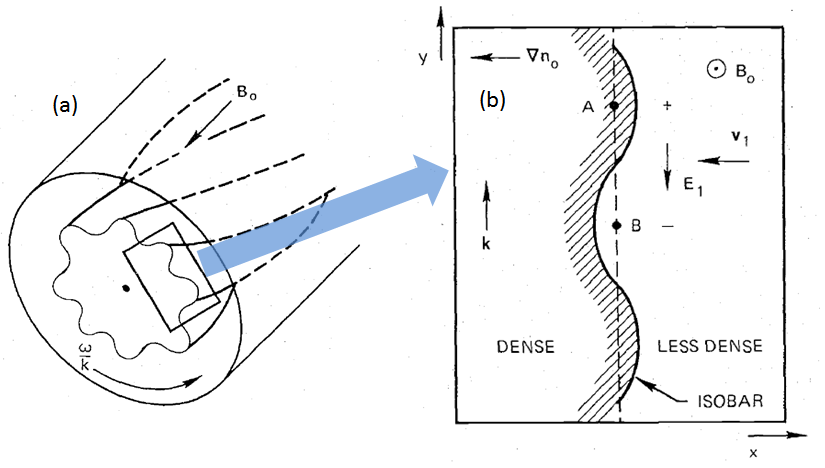
\includegraphics[scale=0.4]{drift_wave.png}
\par\end{centering}
\caption[Physical mechanism of the drift waves]{Physical mechanism of the drift waves. (a) is an enlarged part from (b) the cross section in a cylindrical geometry. Adapted from \cite{Chen_2006_Plasma}}\label{fig:drift_wave}
\end{figure}
%%%%%%%%%%%%%%%%%%%%


Consider now the case when $n_1$ and $v_1$ are out of phase, which can be caused by various mechanisms such as the plasma resistivity. The resistivity effect makes the potential perturbation $\phi_1$ lag behind the density perturbation $n_1$. This phase lag causes $\boldsymbol{v}_1$ to be outward where the plasma has already been shifted outward and the perturbation grows.


\subsection{Microinstabilities in the core region}

Many types of drift wave instabilities can coexist in fusion plasmas. In the core region, the dominating instabilities are trapped electron modes (TEM), ion temperature gradient (ITG) modes, and electron temperature gradient (ETG) modes. The typical wavenumber scales of these modes are shown in figure \ref{fig:turb_scale}.

%%%%%%%%%%%%%%%%%%%%
\begin{figure}[h]
\begin{centering}
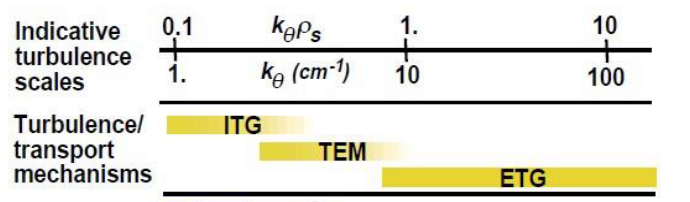
\includegraphics[scale=0.55]{turb_scale.png}
\par\end{centering}
\caption{Spatial scale of ITG, TEM and ETG instabilities in wavenumber and normalized wavenumber.}
\label{fig:turb_scale}
\end{figure}
%%%%%%%%%%%%%%%%%%%%


TEM and ITG are driven by the electron temperature gradient $R/L_{T_e}$ and the ion temperature gradient $R/L_{T_i}$, respectively. Here, $L_{T_e}$ and $L_{T_i}$ are the electron and ion temperature scale length ($L_{T_s}=-T_s/\nabla T_s, s=i,e$). Accordingly, TEM has its phase velocity in the electron diamagnetic direction and ITG has a phase velocity in the ion diamagnetic direction. The stabilization of the modes is also related to the electron density gradient $R/L_{n_e}$, with $L_{n_e}=-n_e/\nabla n_s$ the density scale length. The stability diagram of TEM and ITG is shown in figure \ref{fig:stability_range}, reflecting the complicated interactions and transitions between the two instabilities \cite{Garbet_NF_10_gyrokinetic}.


%%%%%%%%%%%%%%%%%%%%
\begin{figure}[h]
\begin{centering}
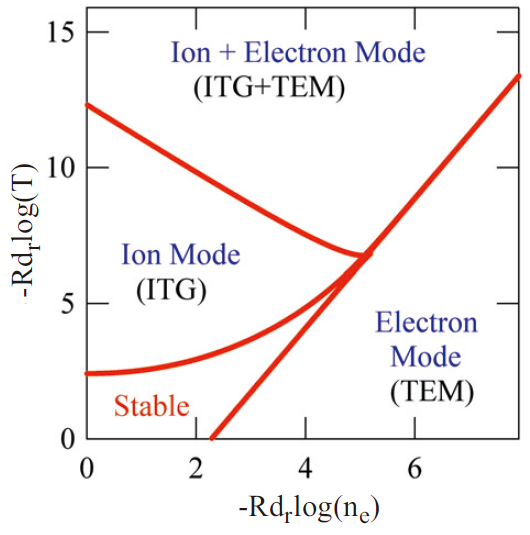
\includegraphics[scale=0.45]{stability_range.png}
\par\end{centering}
\caption[Stability range of ITG and TEM]{Stability range of ITG and TEM under the condition $T_e=T_i$. Adapted from \cite{Garbet_ITGTEM_2004_PPCF_EPS}.}
\label{fig:stability_range}
\end{figure}
%%%%%%%%%%%%%%%%%%%%

One important issue in studying turbulence in fusion plasmas is to identify the dominating plasma instability, depending on plasma conditions. From figure \ref{fig:turb_scale}, TEM and ITG are partly overlapping in terms of wavenumber, making it difficult to distinguish between them. An effective experimental technique to discriminate among TEM and ITG is through the so-called thermodiffusion term in the particle transport analysis \cite{Bourdelle_2007_PoP_Qualikiz}. From \eqref{eq:turb_flux}, both the turbulence equipartition (TEP) and the thermodiffusion term contribute to the convection velocity $V_{turb}$. The TEP term (the curvature pinch) is always directed inwards, whereas the thermodiffusion term can be directed outwards when TEM are dominant and inwards when ITG modes are dominant \cite{Bourdelle_PPCF_05_review_turbulent_particle_transport}.


With a much larger wavenumber, ETG modes can be easily distinguished from the other two instabilities. Moreover, since ETG modes usually make a weaker contributions to the radial transport due to their small scales \cite{Garbet_2001_PPCF} and the high wavenumber is beyond the capability of the diagnostic systems used in this study, we will focus on TEM and ITG hereafter.


%Specifically, a quasi-coherent structure in frequency spectra has been proved to be an explicit indicator of TEM instability in the LOC regime \cite{Arnichand_2015_Thesis, Zhong_2016_PoP, Lee_2018_PoP}. In this thesis, the link is extended to the other components in spectra in both Ohmic and L-mode plasmas, which is discussed in Chapter \ref{ch:ICRH_LH}.


\subsection{Effects of collisions} \label{sec:effect_collision}


Collisions have been found to have a crucial impact on the determination of the micro-instabilities \cite{Vermare_PoP_2011_collisionality_TEM}, since collisions can affect the trapped particle modes via the detrapping mechanism, i.e. collisions tend to stabilize the TEM modes. Among various definitions of collisionality, the effective collisionality ($\nu_\mathrm{eff}$) for drift wave instabilities has been adopted as an excellent indicator for TEM stabilization. It is defined as the ratio between the electron-ion collision frequency and the curvature drift frequency: $\nu_\mathrm{eff} = \nu_\mathrm{ei}/\omega_\mathrm{De}$ \cite{Angioni_2003_PoP,Garbet_ITGTEM_2004_PPCF_EPS}. For ITG and TEM instabilities, the curvature drift frequency provides an estimate of the mode growth rate, and is defined as $\omega_\mathrm{De} = 2 k_{\perp}\rho_Lc_s/R$, with $k_\perp$ the perpendicular wave number, $\rho_\mathrm{L}$ the ion Larmor radius, $R$ (m) the major radius and $c_\mathrm{s}$ the ion acoustic velocity.  Accordingly, $\nu_\mathrm{eff}$ has been approximated as follows \cite{Angioni_2003_PoP,Conway_2006_NF}:%
%%%%%%%%%%%%%%%%%%%%
\begin{equation}\label{eq:nu_eff}
  \nu_\mathrm{eff} \approx 0.1\,R\,Z_\mathrm{eff}\,n_\mathrm{e}\,T_\mathrm{e}^{-2},
\end{equation}
%%%%%%%%%%%%%%%%%%%%
\noindent where $Z_\mathrm{eff}$ is the effective charge number, $n_\mathrm{e}$ (10$^{19}$ m$^{-3}$) the electron density and $T_\mathrm{e}$ (keV) the electron temperature. In this approximation, the normalized perpendicular wave number $k_{\perp}\rho_L$ has been estimated to be $\sqrt{0.1}$, which is the characteristic value for core density fluctuations.


In Ohmic plasmas, the transition from the LOC to SOC confinement regime has been attributed in previous studies to a change in the dominant instability from TEM to ITG modes \cite{Angioni_PoP_2005_LOCSOC_TEMITG,Erofeev_2017_NF}. Experimentally, this connection between confinement regime and dominant micro-instability has also been studied through the dependence of the density peaking on the collisionality in various devices such as Alcator C-Mod and ASDEX Upgrade \cite{Rice_2012_PoP,Lebschy_2018_NF} in both L-mode and H-mode plasmas. The density peaking can be seen as a signature of turbulent pinch velocity. A net inward turbulent pinch gives rise to a peaked density profile with large density peaking and a net outward pinch leads to a flat profile with small density peaking. %Therefore, when electron heating dominates (TEM dominates), the outward thermodiffusion term can become stronger than the inward pinch (both neoclassical and turbulence equipartition) and a flat (or even hollow) density profile appears. In contrast, when ion heating dominates (ITG dominates), the net inward pinch is reinforced and the density profile becomes more peaked.


Figure \ref{fig:turb_nu_eff} (b) shows the evolution of density peaking with effective collisionality ($\nu_\mathrm{eff}$) at different safety factors. At lower $\nu_\mathrm{eff}$, when TEM instability dominates, the density peaking decreases rapidly with $\nu_\mathrm{eff}$, whereas at higher $\nu_\mathrm{eff}$ when TEM may be stabilized, the trend in the density peaking becomes weak and reaches saturation. This may indicate a transition between two turbulence regimes, with a threshold around $\nu_\mathrm{eff} = 1$. Since the effective collisionality is influenced by density, temperature and ion effective charge number, the trends in \ref{fig:turb_nu_eff} (b) is more clear than in \ref{fig:turb_nu_eff} (a), where only the change of density is considered.


%%%%%%%%%%%%%%%%%%%%
\begin{figure}[h]
\begin{centering}
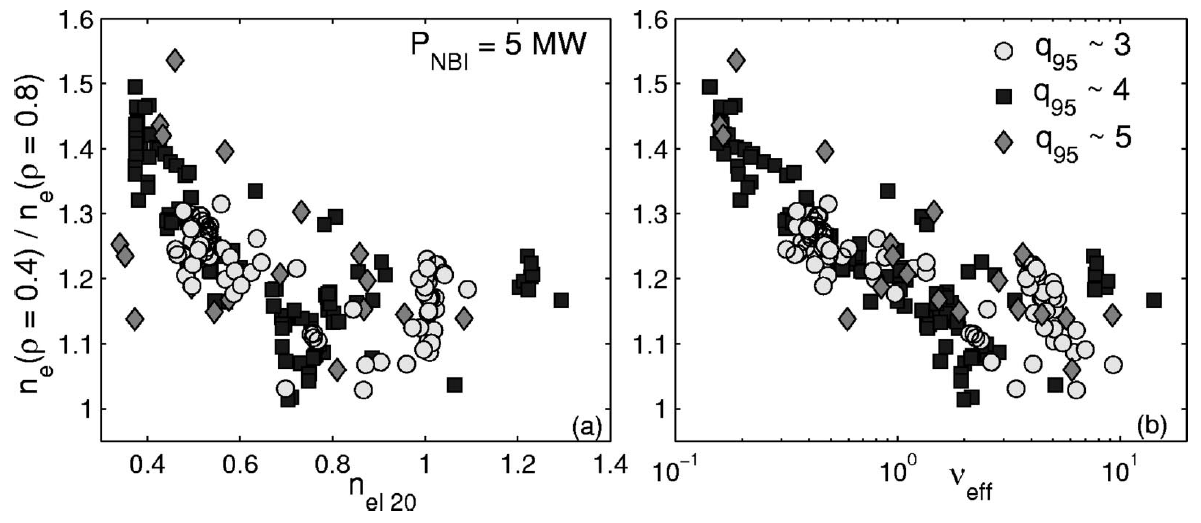
\includegraphics[scale=0.45]{nu_eff.png}
\par\end{centering}
\caption{Evolution of density peaking with (a) the density and (b) collisionality with NBI in ASDEX Upgrade. Adapted from \cite{Angioni_2003_PoP}.}\label{fig:turb_nu_eff}
\end{figure}
%%%%%%%%%%%%%%%%%%%%


\subsection{Turbulence saturation and suppression}

In the linear growth phase, where the increase of the free energy is driven by strong gradients, the magnitude of drift wave instabilities increases, while the linear damping decreases. After the magnitude reaches a threshold, nonlinear interactions appear such as the wave-wave coupling, when $\omega = \omega_1 \pm \omega_2$ or $\bu{k} = \bu{k}_1 \pm \bu{k}_2$. Finally, the nonlinear phase develops into a saturated turbulent state. Different from turbulence in fluids, the parameters in plasma turbulence in tokamaks are usually around the density and temperature threshold. This could be due to the existence of zonal flows (ZFs), which exhibit complex interaction with turbulence through the predator-prey model \cite{Diamond_ZF_2005_PPCF}.

ZFs are symmetric in both poloidal and toroidal direction, in other words, ZFs have finite wavenumber only in the radial direction. They are elongated vortex modes with zero frequency, which make it very difficult to detect them. From the theoretical point-of-view, zonal flows are generated by turbulence, but they have a suppressing effect on turbulence generation and propagation. ZFs can break the turbulent eddies into smaller ones and thus greatly reducing their radial transport. Other turbulence suppression effects are velocity shear from plasma rotation and magnetic shear by constructing proper profiles of the safety factor (or plasmas current).


\section{Density fluctuations} \label{sec:properties_of_density_fluctuations}

In the saturated (fully developed) state, turbulence can induce fluctuations of various plasma parameters, such as $\delta n$, $\delta T$, $\delta\phi$ and $\delta$\textbf{B}. Most measurements of turbulence rely on $\delta n$ due to the higher sensitivity of diagnostics than the other fluctuations.


\subsection{Radial profiles of the fluctuation level}

The density fluctuation level $\delta n$ is very important due to its direct link with confinement performance. The relative magnitude $\delta n/n$ is usually connected with different confinement regimes. Many studies have been dedicated to the determination of $\delta n/n$ under various plasma conditions and heating scenarios.


%%%%%%%%%%%%%%%%%%%%
\begin{figure}[h]
\begin{centering}
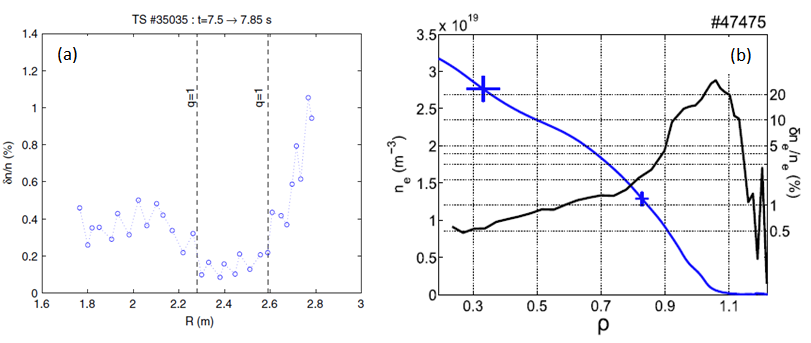
\includegraphics[scale=0.7]{fluc_level_ohmic.png}
\par\end{centering}
\caption{Density fluctuation level in the (a) core and (b) edge region in Tore Supra ohmic discharges. From \cite{Sabot_2006_NF, Greg_PhD_thesis}.}
\label{fig:fluc_level_ohmic}
\end{figure}
%%%%%%%%%%%%%%%%%%%%


Figure \ref{fig:fluc_level_ohmic} shows the radial profile of $\delta n/n$ in Ohmic plasmas. The complete radial profile, from the LFS through the center to the HFS, of $\delta n/n$ measured by fixed-frequency reflectometry is shown in figure \ref{fig:fluc_level_ohmic} (a). It is clear that $\delta n/n$ remains at a low level ($< 0.2\%$) near the central region, especially inside the $q = 1$ surface, where linear turbulence dominates. Towards the edge region, $\delta n/n$ increases rapidly and specifically at the LFS near the edge $\delta n/n$ can be larger than $1 \%$. At the HFS, $\delta n/n$ remains at a moderate level. Figure \ref{fig:fluc_level_ohmic} (b) shows the profiles of density ($n$) and density fluctuation level (\ref{fig:fluc_level_ohmic}) measured by fast-sweeping reflectometry in the edge region for another discharge. From the core region to the edge region, $\delta n/n$ first increases slowly, then rapidly near the last-closed magnetic surface ($\rho \sim 1$), which is consistent with the observations in figure \ref{fig:fluc_level_ohmic} (a).

Furthermore, $\delta n/n$ with different heating scenarios is shown in figure \ref{fig:fluc_level_heating}. With auxiliary heating, $\delta n/n$ still increases from the center to the edge, but the magnitude of $\delta n/n$ is systematically higher at all radial positions. Comparing the pure ICRH ($P_\mathrm{ICRH} = 4.7$ MW) with the mixed heating scheme ($P_\mathrm{ICRH} + P_\mathrm{LH} = 4$ MW), the effect of ICRH turns out to be stronger than that of LH heating.



%%%%%%%%%%%%%%%%%%%%
\begin{figure}[!h]
\begin{centering}
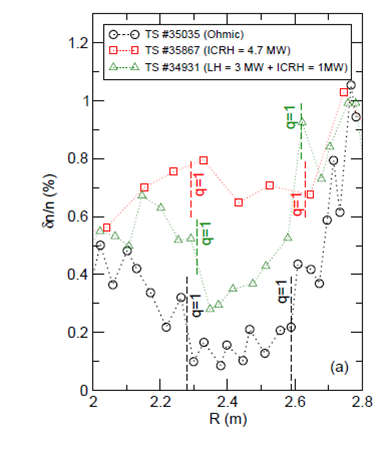
\includegraphics[scale=0.6]{fluc_level_heating_2.png}
\par\end{centering}
\caption{Density fluctuation level with auxiliary heating methods compared with the Ohmic plasmas. From \cite{Sirinelli_2006_Thesis}.}
\label{fig:fluc_level_heating}
\end{figure}
%%%%%%%%%%%%%%%%%%%%


\subsection{Diagnostics for density fluctuations}

Although the above profiles of the density fluctuation level have been measured by reflectometry diagnostics, many other diagnostic methods have been developed for measuring density fluctuations. Every diagnostic has its specific working conditions and limitations.

Langmuir probes (LPs) are the simplest and most accurate measurement technique, able to measure fluctuations of $n$, $T$ and $\phi$ simultaneously. By measuring the fluctuation of saturation currents $\widetilde{I_{sat}}$, one can obtain directly the density fluctuations $\widetilde{n}$. Although LPs have been widely used in low-temperature plasmas, their application in tokamaks is restricted to the edge region, due to the hostile plasma conditions. Even the improved fast-reciprocating LP can only be inserted a few centimeters deeper, but can not reach the central plasma region. Other diagnostics such as heavy ion beam probes (HIBP) and beam emission spectroscopy (BES) have been developed to detect density fluctuations in the core region, but they can probe only a limited spatial range and have limited accuracy and spatial resolution \cite{Bretz_1997_RSI}.

On the other hand, reflectometry is a versatile diagnostic, able to measure $\widetilde{n}$ at multiple positions with high spatial and temporal resolution. By measuring the phase fluctuation $\widetilde{\phi}(t)$ in the acquired signal, the density fluctuations $\widetilde{n}(t)$ can be obtained through a transfer function. Moreover, by using multiple antennas and a correlation technique (see appendix \ref{appA}), reflectometry can also provide the energy distribution from the power or wavenumber spectra, as well as the correlation length and time of the turbulent eddies, and the rotation of the turbulence structures. These advantages make reflectometry a powerful diagnostic tool for studying turbulence in fusion plasmas. The details of reflectometry are presented in the next chapter.

